\documentclass{article}[12pt]
\usepackage{fontspec}   %加這個就可以設定字體
\usepackage{xeCJK}       %讓中英文字體分開設置
\usepackage{indentfirst}
\usepackage{listings}
\usepackage[newfloat]{minted}
\usepackage{float}
\usepackage{graphicx}
\usepackage{caption}
\usepackage{fancyhdr}
\usepackage{hyperref}
\usepackage{amsmath}
\usepackage{multirow}
\usepackage[dvipsnames]{xcolor}
\usepackage{graphicx}
\usepackage{tabularx}
\usepackage{booktabs}
\usepackage{caption}
\usepackage{subcaption}
\usepackage{pifont}
\usepackage{amssymb}

\usepackage[breakable, listings, skins, minted]{tcolorbox}
\usepackage{etoolbox}
\setminted{fontsize=\footnotesize}
\renewtcblisting{minted}{%
    listing engine=minted,
    minted language=python,
    listing only,
    breakable,
    enhanced,
    minted options = {
        linenos, 
        breaklines=true, 
        breakbefore=., 
        % fontsize=\footnotesize, 
        numbersep=2mm
    },
    overlay={%
        \begin{tcbclipinterior}
            \fill[gray!25] (frame.south west) rectangle ([xshift=4mm]frame.north west);
        \end{tcbclipinterior}
    }   
}

\usepackage[
  top=2cm,
  bottom=2cm,
  left=3.5cm,
  right=3.5cm,
  headheight=17pt, % as per the warning by fancyhdr
  includehead,includefoot,
  heightrounded, % to avoid spurious underfull messages
]{geometry} 

\newenvironment{code}{\captionsetup{type=listing}}{}
\SetupFloatingEnvironment{listing}{name=Code}


\title{人工智慧概論 HW2 報告}
\author{110550088 李杰穎}
\date{\today}

\setCJKmainfont{Noto Serif TC}
\setmonofont[Mapping=tex-text]{Consolas}

\XeTeXlinebreaklocale "zh"             %這兩行一定要加,中文才能自動換行
\XeTeXlinebreakskip = 0pt plus 1pt     %這兩行一定要加,中文才能自動換行

\setlength{\parindent}{0em}
\setlength{\parskip}{2em}
\renewcommand{\baselinestretch}{1.5}
\begin{document}

\maketitle

\section{Preprocessing}
在本次作業中,我主要實作了以下幾種 preprocessing 的方法,條列如下:
\begin{enumerate}
    \item 將英文大寫轉成小寫: 使用 Python 內建的 \texttt{lower()} 函式,將字串文字全部
    轉成小寫
    \item 移除 stopwords: 利用 nltk 提供的 stopwords 列表,將 stopwords 從字串中移除。
    \item 移除 \texttt{<br />} HTML tag: 使用 Python 內建的 \texttt{replace()} 函式,
    將 \texttt{<br />} 用一個空白取代
    \item 移除標點符號: 利用 for 迴圈檢查每一個 char 是否為標點符號,如果非標點符號則將其加進一個 list,
    最後再使用 \texttt{``".join()} 來將 list 內元素轉為字串。檢查標點符號的部分則使用內建之
    \texttt{string.punctuation} 來檢查。
    \item Stemming (使用 nltk 內建之 SnowballStemmer): Stemming (詞幹提取) 是一種將詞彙去除後綴的方式。
    將單字進行 stemming 會讓模型不用處理額外的訊息,以下是一些經過 SnowballStemmer 處理後的單字。\\
    cared $\rightarrow$         care, 
    university $\rightarrow$     univers, 
    fairly $\rightarrow$         fair, 
    easily $\rightarrow$         easili,
    singing $\rightarrow$       sing, 
    sings $\rightarrow$         sing,  
    sung  $\rightarrow$          sung,  
    singer $\rightarrow$        singer,  
    sportingly $\rightarrow$     sport
\end{enumerate}

在進行 preprocessing 時,會依照上面排列的順序進行這五個步驟。

下方為一英文句子通過以上 preprocessing 後的句子。

``It is a truth universally acknowledged that<br /> 
a single man in possession of a good fortune must be in want of a wife." $\rightarrow$
``truth univers acknowledg singl man possess good fortun must want wife"

我也會在下文討論各 preprocessing 的方法對於最終的 F1-Score 的影響。

\section{Implement the bi-gram language model}

本部分介紹 bi-gram model 的實作,因為大部分實作細節都可以在繳交的程式碼中看到,故在此
我只大致說明實作內容。

\begin{enumerate}
    \item 計算各 uni-gram 及 bi-gram 的出現頻率: 由於在計算 $P(w_i|w_{i-1})$ 時,需要同時知道 bi-gram 及
    uni-gram 的出現頻率,故先 iterate 所有 document 並利用 dict 來統計出現的頻率。
    \item 利用上一個步驟的頻率求出 $P(w_i|w_{i-1})$: 左述之條件機率可由下式得到:
    \begin{equation}
        \label{eq: P}
        P(w_i|w_{i-1}) = \frac{\text{count}(w_{i-1}, w_i)}{\text{count}(w_{i-1})}
    \end{equation}
    \item 將所有算出的機率利用 Python 內建的 dict 資料結構,
    存為 \texttt{model[$w_{i-1}$][$w_i$]} 的形式,而 feature 則儲存各 bi-gram
    的頻率 (即為 \texttt{feature[($w_{i-1}$, $w_i$)]})
\end{enumerate}

可以發現若 Eq. \ref{eq: P} 中分子及分母若為 0,則會使機率的計算發生問題
(如 \texttt{ZeroDivisionError: division by zero}),
於是我在此使用 Add-1 (Laplace) Smoothing 來避免以下問題,Add-1 Smoothing 的具體式子如下:

\begin{equation}
    \label{eq: add-1}
    P(w_i|w_{i-1}) = \frac{\text{count}(w_{i-1}, w_i) + 1}{\text{count}(w_{i-1}) + |V|}
\end{equation}

根據網路上查到的資料, $|V|$ 為 unique vocabulary 的數量。在使用 Add-1 Smoothing 後,就不會出現先前
機率出現 0 或無限大的情形。

但值得注意的是,我自行測試後發現,當使用 bi-gram model 時,利用上述定義計算出來的 perplexity 相當大,
約為 2312 左右。
這個數值是相當不合理的,與 uni-gram 模型進行比較,uni-gram 模型的 perplexity 僅為 914。
當 n-gram 的 n 值越大時,其 perplexity 應該會隨之降低。我與同學討論過後,認為 Add-1 smoothing 中 $|V|$
的定義應該為:

\begin{equation}
    \label{eq: v}
    |V_{w_{i-1}}| = \text{\# of unique bi-grams that start with } w_{i-1}
\end{equation}

根據以上定義,重新計算 bi-gram model 的 perplexity 後,其數值降低為 174 ,相較於 2312 是一個較為合理的數值。

\section{Feature Selection}

我主要使用使用了兩種 feature selection 的方法,第一種方法是按 bi-gram 的
出現頻率進行排序。第二種則是 Chi-Square Test 進行 feature selection。第一種方式較為簡單,在此不在贅述。
接下來會介紹 Chi-Square Test 的實做細節。

\subsection{Chi-Square Test Feature Selection}
$\chi^2$ 是一個可以計算出特定 feature 對於最終答案 dependent 程度的演算法,對於二元分類問題
其計算方式如下:

\begin{align*}
    e_{00}(\text{bi-gram}) &= \frac{sum_{neg}(sum_{pos}+sum_{neg}-(N_{pos}(\text{bi-gram})+N_{neg}(\text{bi-gram})))}{sum_{pos}+sum_{neg}} \\
    e_{01}(\text{bi-gram}) &= \frac{sum_{pos}(sum_{pos}+sum_{neg}-(N_{pos}(\text{bi-gram})+N_{neg}(\text{bi-gram})))}{sum_{pos}+sum_{neg}} \\
    e_{10}(\text{bi-gram}) &= \frac{sum_{neg}(N_{pos}(\text{bi-gram})+N_{neg}(\text{bi-gram}))}{sum_{pos}+sum_{neg}} \\
    e_{11}(\text{bi-gram}) &= \frac{sum_{pos}(N_{pos}(\text{bi-gram})+N_{neg}(\text{bi-gram}))}{sum_{pos}+sum_{neg}} \\
\end{align*}
\begin{equation}
    \begin{aligned}
        \chi^2(\text{bi-gram}) = &\frac{(sum_{neg} - N_{neg}(\text{bi-gram}) - e_{00}(\text{bi-gram}))^2}{e_{00}(\text{bi-gram})} \\
        &+ \frac{(sum_{pos} - N_{pos}(\text{bi-gram}) - e_{01}(\text{bi-gram}))^2}{e_{01}(\text{bi-gram})} \\
        &+ \frac{(N_{neg}(\text{bi-gram}) - e_{10}(\text{bi-gram}))^2}{e_{10}(\text{bi-gram})} \\
        &+ \frac{(N_{pos}(\text{bi-gram}) - e_{11}(\text{bi-gram}))^2}{e_{11}(\text{bi-gram})}
    \end{aligned}    
\end{equation}

其中 $sum_{pos}$ 為 positive 句子中的 bi-gram 總和,
$sum_{neg}$ 為 negative 句子中的 bi-gram 總和。
$N_{pos}(\text{bi-gram})$ 為 $\text{bi-gram}$ 在 positive 句子出現的次數,
$N_{neg}(\text{bi-gram})$ 為 $\text{bi-gram}$ 在 negative 句子出現的次數。

透過以上方式可以計算出特定 bi-gram 的 $\chi^2$ score。$\chi^2$ score 越高,代表此 bi-gram
對於結果越 dependent,也就代表此 bi-gram 越有價值。

計算出所有 bi-gram 的 $\chi^2$ score 後,我們就可以將各 bi-gram 透過 $\chi^2$ score 從大
排到小,並取出前 \texttt{feature\_num} 個 bi-gram 做為 GaussianNB 的輸入。

\section{Perplexity}
透過 Eq. \ref{eq: add-1}, \ref{eq: v},我們即可以計算一個 bi-gram 模型的 perplexity,perplexity 的計算方式
如下:

\begin{equation}
    \text{Perplexity} = 2^{-\text{entropy}}, \text{where entropy} = \frac{1}{N} \sum^{N}_{i=0} \log_{2}(P(w_i|w_{i-1}))
\end{equation}

當我們使用測試資料去測試模型時,算出的 perplexity 越低時,代表模型認為測試資料中的句子出現的機率越高。
也就是說當一個語言模型的 perplexity 越低時,模型的 performance 越好。

\section{實驗和比較}

\subsection{Preprocessing 相關實驗}
此部分會探討不同 preprocessing 的方法對於 perplexity, F1-score, precision 及 recall
的影響。

本次作業中,我主要實作了四種 preprocessing 的方法,並透過結合這四種方法,訓練出了七種不同的 bi-gram 模型 
(feature 數量固定為 500,且使用 Chi-Square test feature selection、皆轉成小寫),
其 performance 如下表:

\begin{table}[H]
    \centering
    \caption{不同 preprocessing 的組合之 perplexity 及 F1-score}
    \begin{tabular}{|c|c|c|c|c|c|}
    \hline
    Remove \textless{}br /\textgreater{} & Remove stopwords & Remove punctuations & Stemming & Perplexity       & F1-score        \\ \hline
                                         &                  &                     &          & \textbf{134.287} & 0.7596          \\ \hline
    \checkmark                                   &                  &                     &          & 148.447          & 0.765           \\ \hline
    \checkmark                                   & \checkmark               &                     &          & 320.902          & 0.7379          \\ \hline
    \checkmark	                                   &                  & \checkmark                  &          & 172.528          & 0.7787          \\ \hline
    \checkmark                                   &                  &                     & \checkmark       & 152.991          & 0.7797          \\ \hline
    \checkmark                                   & \checkmark               & \checkmark                  & \checkmark       & 433.002          & 0.7371          \\ \hline
    \checkmark                                   &                  & \checkmark                  & \checkmark       & 174.381          & \textbf{0.7881} \\ \hline
    \end{tabular}
\end{table}

可以發現 performance 最高的 preprocessing 方法為為轉為小寫 + 移除 br + 標點符號 + SnowballStemmer,
其 F1-score 為 0.7881。下文若有提到 preprocessing 則我都是使用此種方式。

值得注意的是,perplexity 與 F1-score 並沒有明顯的相關性,當 perplexity 越低時,F1-score 並不會跟著升高,
反之亦然。例如在上表中,perplexity 最低的是未經過任何 preprocessing 的模型。
這可能是因為 perplexity 本身是用來量測 test set 的句子在經過 train set 訓練的模型來說,這個句子的通順程度。
這個量測方法對於文本情緒的判斷是毫無關聯的,這可能就是為什麼我們量測出 perplexity 與 F1-score 幾乎無關的原因。


\subsection{Feature Selection 相關實驗}
此部分會探討不同 feature selection 的方式對於 perplexity, F1-score, precision 及 recall
的影響。

在本次作業中,我主要實作了兩種 feature selection 的方法:

\begin{enumerate}
    \item 將出現頻率最高的 bi-gram 作為 feature (Sorted Feature)
    \item 上文中提到的 Chi-Square Test
\end{enumerate}

以下實驗皆固定 feature 數量為 500,preprocessing 方法為移除 br + 標點符號 + SnowballStemmer
,並都為 bi-gram 模型。

\begin{table}[H]
    \centering
    \caption{兩種不同 feature section 的 F1-score, Precision 及 Recall}
    \begin{tabular}{@{}cccc@{}}
    \toprule
    Method          & F1-score        & Precision       & Recall          \\ \midrule
    Sorted Features & 0.7259          & 0.7278          & \textbf{0.7911} \\
    Chi-Square Test & \textbf{0.7881} & \textbf{0.8084} & \textbf{0.7911} \\ \bottomrule
    \end{tabular}
\end{table}

可以發現使用 Chi-Square Test 的 bi-gram 模型表現較佳,這也符合我的預期。
Chi-Square Test 的執行時間不長,在我的電腦上大約只需運行 10 分鐘左右。

下表為兩種 feature selection 方法所挑出的前 20 個 features。

% Please add the following required packages to your document preamble:
% \usepackage{booktabs}
\begin{table}[H]
    \centering
    \caption{兩種不同 feature section 的前 20 個 features}
    \begin{tabular}{@{}cc@{}}
    \toprule
    \textbf{Sorted Features} & \textbf{Chi-Square Test} \\ \midrule
    ('of', 'the')            & ('the', 'worst')         \\
    ('in', 'the')            & ('wast', 'of')           \\
    ('this', 'movi')         & ('a', 'great')           \\
    ('the', 'film')          & ('the', 'best')          \\
    ('and', 'the')           & ('is', 'a')              \\
    ('is', 'a')              & ('worst', 'movi')        \\
    ('the', 'movi')          & ('so', 'bad')            \\
    ('to', 'be')             & ('suppos', 'to')         \\
    ('to', 'the')            & ('look', 'like')         \\
    ('this', 'film')         & ('at', 'all')            \\
    ('it', 'is')             & ('the', 'onli')          \\
    ('this', 'is')           & ('this', 'movi')         \\
    ('on', 'the')            & ('high', 'recommend')    \\
    ('in', 'a')              & ('bad', 'movi')          \\
    ('it', 'was')            & ('wast', 'your')         \\
    ('one', 'of')            & ('not', 'even')          \\
    ('for', 'the')           & ('a', 'bad')             \\
    ('with', 'the')          & ('worst', 'film')        \\
    ('of', 'a')              & ('a', 'wast')            \\
    ('is', 'the')            & ('your', 'time')         \\ \bottomrule
    \end{tabular}
\end{table}

可以發現使用 sorted feature 方法所挑出來的 feature 大多與文本的情緒無關,
大多數為電影相關的單字及介詞。而使用 Chi-Square Test 方法所挑選出來的 feature 
與文本的情緒高度相關,如 ``worst'', ``great'', ``bad'', ``best'', ``wast(e)'', 
``high recommend'' 等,這些字詞都可以很好的去分類文本。

\subsection{Number of features 相關實驗}
此部分會探討不同 feature 數量對於 perplexity, F1-score, precision 及 recall
的影響。

值得注意的是,此部分中的 features 皆是透過 Chi-Square Test Feature Selection 來選出。

我們分別比較了六種不同 ngram 的模型 (uni/bi/tri-gram, w/ or w/o preprocessing)
在七種 feature 數量 (250、500、750、1000、1500、2000 及 2500) F1-score 數值。
結果整理為下圖。

\begin{figure}[H]
    \centering
    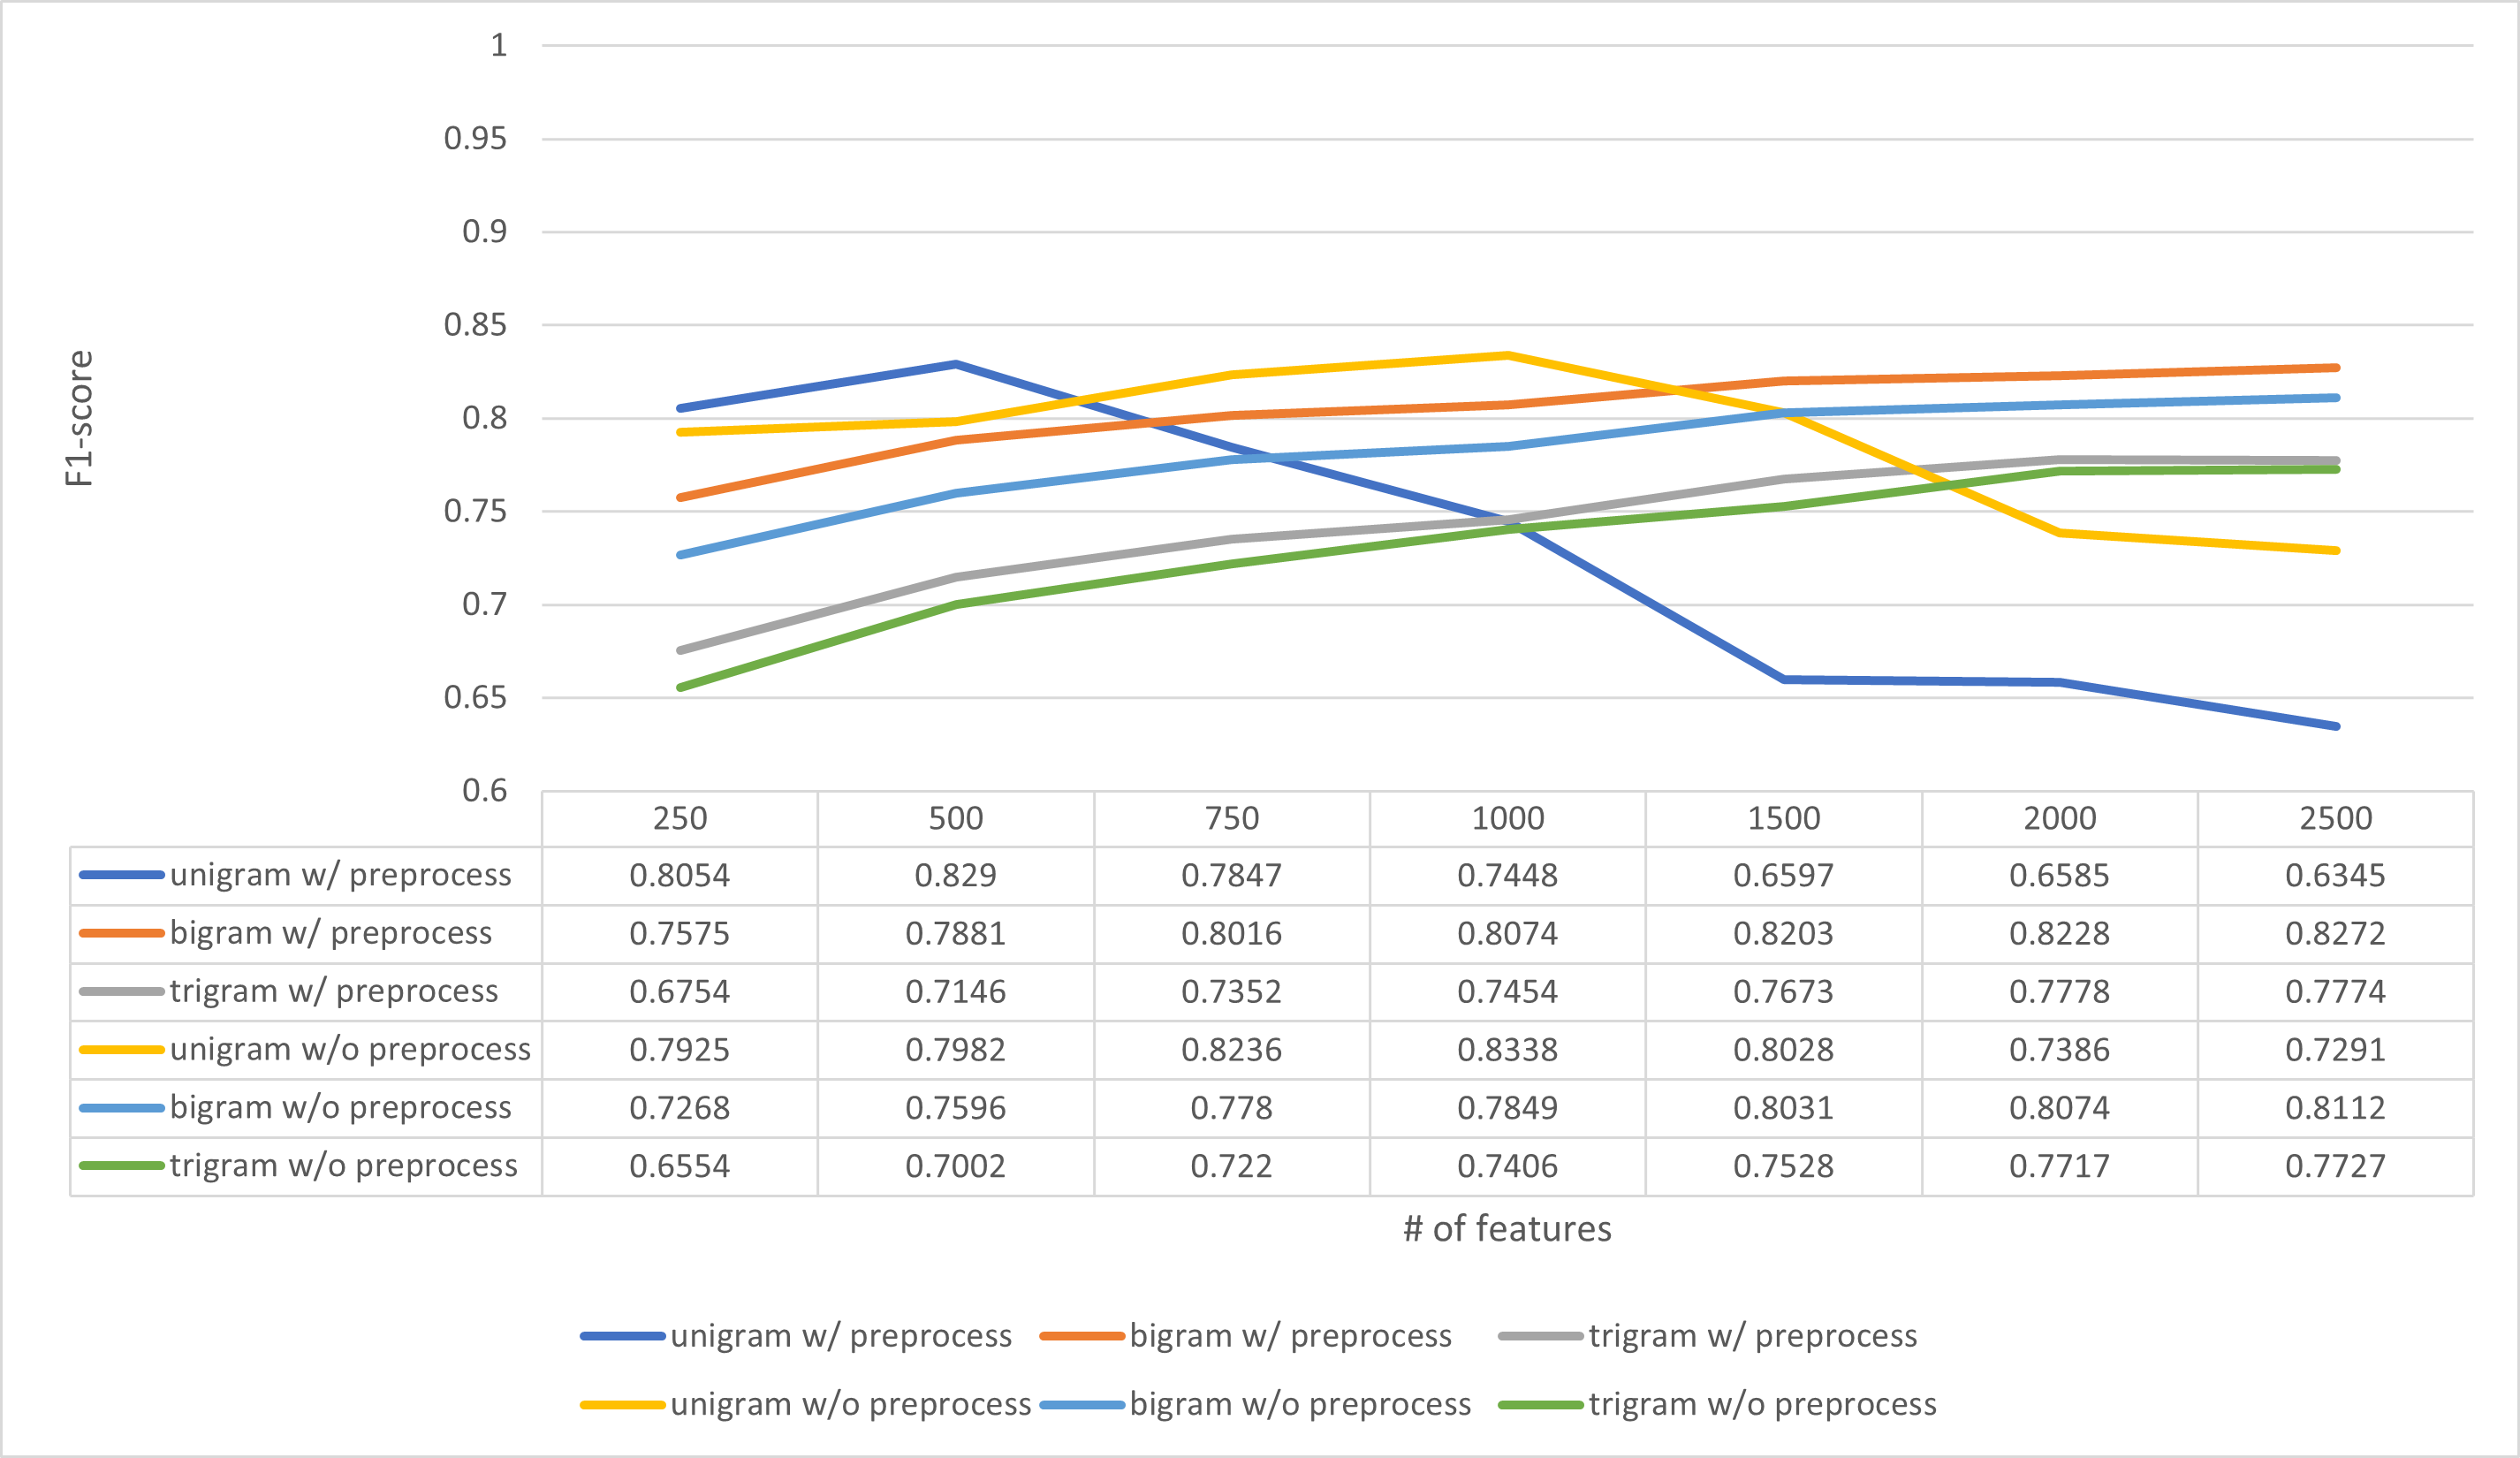
\includegraphics[width=\textwidth]{figure/features.png}
    \caption{六種不同 ngram 的模型 (uni/bi/tri-gram, w/ or w/o preprocessing) 在不同 features 數量下 F1-score 的比較圖}
\end{figure}

可以發現在 featrues 數量為 500 的條件下,經過 preprocessing 的 uni-gram 表現最佳,
其 F1-score 達到 0.8054。而最佳的模型則為 feature 數量 1000 \
且未經過 preprocessing 的 uni-gram 模型,其 F1-score 為 0.8338。



\subsection{Uni-gram, bi-gram, tri-gram 和 DistilBert 相關實驗}
本報告中,我分別實作了 uni-gram, bi-gram 和 tri-gram。在此部分中,我將會將此三種 n-gram 方法與現今
較流行且 performance 較好的 BERT 進行比較。

我分別測試了 uni/bi/tri-gram 經過 preprocessing 的模型,feature 數量固定為 500,
並將其與 w/ 和 w/o preprocessing 的 DistilBert 進行比較,下圖為 F1-score 之比較表:

% Please add the following required packages to your document preamble:
% \usepackage{booktabs}
\begin{table}[H]
    \centering
    \caption{六種不同 model 的 F1-score}
    \begin{tabular}{@{}cc@{}}
    \toprule
    \textbf{Model}                                 & \textbf{F1-score} \\ \midrule
    uni-gram                                       & 0.829             \\
    bi-gram                                        & 0.7881            \\
    tri-gram                                       & 0.7146            \\
    BERT w/o preprocessing                         & 0.9337   \\
    BERT w/ preprocessing                          & 0.9129            \\
    BERT only remove \textless{}br /\textgreater{} & \textbf{0.9372}            \\ \bottomrule
    \end{tabular}
\end{table}

可以發現在 n-gram 模型中,uni-gram 的 performance 最佳,其 F1-score 為 0.829,我猜想原因可能因為在本任務中,判斷一個文本是否正面其實不太需要前後文的結構,只需要抓出
關鍵字如 ``best'', ``worst'' 即可以判斷一個文本的情緒。在需要額外透過前後文的來判斷
情緒的情況中,一般的 bi-gram 及 tri-gram 模型也沒辦法處理複雜的前後文,故簡單的 uni-gram 
模型即可以很好的處理此任務。

值得注意的是,DistilBert 在經過 preprocessing 後,F1-score 反而還變得比較低,
於是我又在另外訓練一個只將 <br /> tag (不轉成小寫) 移除的模型,可以發現其 performance 是最好的,
F1-score 為 0.9372。

我認為其原因可能是因為 DistilBert 本身就可以判斷哪些字詞是可以用來判斷情緒,哪些是不行的,移除所有標點符號和
進行 stemming 可能會失去過多語料資訊,使 DistilBert 的表現較差。


\section{討論}
\subsection{Why bi-gram can't outperform DistilBert}

BERT 使用了一種稱為 self-attention 的機制,能去自動偵測句子中哪些字詞是與答案有關,哪些則無關
,也可以辨識出句子的前後語義。

而 bi-gram 模型的基本上只能考慮相鄰兩個字詞的關係,
且在本次作業中在進行 BERT 的訓練時,我們也利用 GPU 來進行加速,
雖然計算的時間可能是差不多的,
但如果考慮兩者的計算量,其差距是很大的。

\subsection{Why bi-gram can't consider long-term dependencies?}

因為 bi-gram 模型只會考慮相鄰兩個字詞的關係,例如 ``Weather yesterday is nice, but today is bad.'' 和
``Weather yesterday is bad, but today is nice.'' 這兩個句子對於 bi-gram 來說是完全相同的。
但其實兩個句子的語意是完全相反的。

而 BERT 模型則會考慮上下文的語句來做出最後的判斷

\subsection{Would the preprocessing methods improve the performance of the bi-gram model?}

如前文所提到,preprocessing 對於 bi-gram 模型是有幫助的,
這點可以由經過 preprocessing 及未經過 preprocessing 的 perplexity, F1-Score 去佐證。

Preprocessing 可以幫助模型去除掉沒有必要的資訊,
使模型的判斷結果變得更為精準。

\subsection{If convert all words that appeared less than 10 times as [UNK], would it in general
increase or decrease the perplexity on the previously unseen data
compared to an approach that converts only a fraction of the words that
appeared just once as [UNK]?}

將所有出現頻率小於 10 次的字詞轉為 [UNK], 可以讓模型不熟悉的字詞變少,使計算出來的機率升高,entropy 值變小,
perplexity 也就跟著降低。

此種方法相較於只將部分出現一次的字詞轉為 [UNK] 的方法,進一步使低頻率的字詞減少,使得計算出的機率升高。
故 perplexity 相較來說也會比較低。


\section{結論}

在 n-gram 模型中,在 feature 數量固定為 500 的條件下
,performance 最高的為經過 preprocessing 的 uni-gram 模型。

而 BERT 模型的 performance 相較於所有 n-gram 模型來說,可以說非常的高,這可能得益於 BERT 中
的 self-attention 機制。

在文本情緒判斷這個任務中, perplexity 與 F1-score 的相關性並不大,
這可能是因為文本之間的前後文對於情緒的判斷的相關性很小。

在本次作業中,我主要比較了 n-gram 模型與 BERT 模型,並從中學習到如何從頭實作 n-gram model。
過程中對於 add-1 smoothing 中的 $|V|$ 參數也有了自己的看法。

\end{document}